\documentclass{article}
\usepackage{graphicx} % Required for inserting images
\usepackage[italian]{babel}
\usepackage{amsmath}
\usepackage{amssymb}
\usepackage[hidelinks]{hyperref}
\usepackage{xcolor}
\usepackage{float}
\usepackage{caption}
\usepackage{multicol}
\usepackage{algorithm}
\usepackage{algpseudocode}

\newtheorem{theorem}{Teorema}
\newtheorem{lemma}[theorem]{Lemma}

\title{Basi di dati}
\author{Leonardo Ganzaroli}
\date{}

\begin{document}

\maketitle

\addcontentsline{toc}{section}{\protect\numberline{}Introduzione}

\tableofcontents

\newpage

\hypersetup{allcolors=black}

\section*{Introduzione}

Questi appunti sono derivanti principalmente dalle dispense dei corsi \textit{Basi di dati 1 e 2} che ho seguito durante la laurea Triennale di informatica all'università "La Sapienza".\newline

\noindent Il modulo 2 del corso era basato sulla progettazione di un DB nella sua interezza partendo da un documento di specifica, per modellare il tutto si usava una combinazione di UML e FOL che veniva alla fine "tradotto" in SQL. Essendo il tutto estremamente pratico riporto solo la parte teorica della FOL.

\newpage

\part{}

\section{Definizioni}

\textbf{Definizione} Una base di dati è un insieme di file mutualmente connessi.\newline

\noindent\textbf{Definizione} Il DBMS è un insieme di strumenti software atti a gestire grandi quantità di dati.\newline

\noindent\textbf{Definizione} Un sistema informativo è un complesso di dati organizzati in memoria secondaria.\newline

\noindent I dati possono essere:
\begin{itemize}
    \item \textbf{Strutturati}

        Un oggetto viene rappresentato da stringhe di simboli/numeri.

    \item \textbf{Non strutturati}

        Testi in linguaggio naturale.\newline
    
    
\end{itemize}

\noindent Esistono 2 modelli per organizzare i dati:
\begin{enumerate}
    \item \textbf{Logici}

        Indipendenti dalle strutture fisiche.\newline

        Alcuni sono:
        \begin{itemize}
            \item \textbf{Reticolare}

                Ha una struttura a grafo in cui:
                \begin{itemize}
                    \item Nodi = record
                    \item Archi = link
                \end{itemize}

            \item \textbf{Gerarchico}

                Come il precedente ma il reticolo è una foresta.

            \item \textbf{Relazionale}

                Presenta un'organizzazione a tabelle.

            \item \textbf{A oggetti}

                Basato sul concetto di classe.
            
        \end{itemize}

    \item \textbf{Concettuali}

        Indipendenti dalle modalità realizzative, rappresentano le entità del mondo reale e le loro relazioni.
    
\end{enumerate}

\newpage

\noindent I database presentano un'organizzazione a livelli indipendenti che permette di fornire all'utente una vista astratta dei dati:

\begin{figure}[ht]
    \centering
    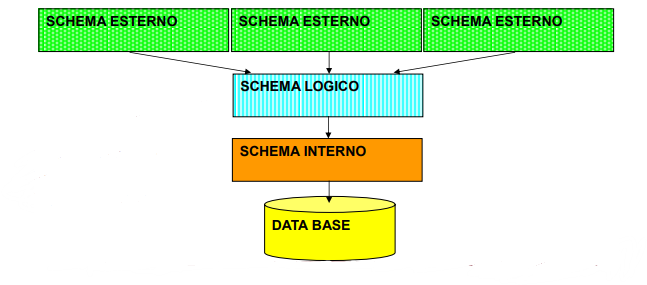
\includegraphics[width=\linewidth]{db.png}
    \caption{Livelli}
    \label{fig:db_liv}
\end{figure}

\begin{itemize}
    \item \textbf{Esterno}

        Fornisce delle "viste" sul contenuto del DB, queste possono mostrare i dati in modo diverso dai livelli sottostanti.

    \item \textbf{Logico}

        L'effettivo modello usato.

    \item \textbf{Interno}

        I file.\newline
    
\end{itemize}

\noindent\textbf{Definizione} Lo schema descrive la struttura del DB.\newline

\noindent\textbf{Definizione} L'istanza è data dai valori attuali presenti nel DB.\newline

\noindent Per poter interagire con il DB si usano i linguaggi:
\begin{itemize}
    \item DDL (per gli schemi)
    \item DML (per le istanze)
\end{itemize}

\noindent Nel caso di DB relazionali il linguaggio standard è l'SQL (racchiude entrambe le funzionalità).

\newpage

\section{Modello relazionale}

In questo modello i dati vengono rappresentati sottoforma di tabelle, esse rappresentano delle relazioni matematiche tra insiemi.\newline

\noindent\textbf{Definizione} Un dominio è un insieme potenzialmente infinito di valori.\newline

\noindent Ogni colonna ha associato un dominio, una riga sarà quindi una n-upla del prodotto cartesiano dei domini. Per fornire un'interpretazione ai dati si associa ad ogni colonna un nome detto attributo che funge anche da identificativo della stessa.\newline

\noindent\textbf{Definizione} Il valore NULL viene usato per indicare mancanza di informazione.\newline

\begin{table}[ht]
    \centering
    \begin{tabular}{c|c|c}
        \textcolor{red}{Nome} & \textcolor{red}{ID} & \textcolor{red}{Data di nascita}\\
         \hline
        \textcolor{blue}{Franco} & \textcolor{blue}{984} & \textcolor{blue}{1/15/96}\\
         \hline
        \textcolor{blue}{Mario} & \textcolor{blue}{987} & \textcolor{blue}{NULL}\\
    \end{tabular}
    \label{tab:rel}
\end{table}

\noindent Gli elementi in \textcolor{red}{rosso} sono gli attributi, considerandoli nel loro insieme ottengo lo schema della relazione. Quelli in \textcolor{blue}{blu} invece sono l'istanza della relazione.\newline

\noindent\textbf{Definizione} Una chiave è uno o più attributi che identificano univocamente una n-upla, nello specifico un insieme di attributi X di una relazione R è chiave se:
\begin{enumerate}
    \item Per ogni istanza di R non esistono 2 n-uple distinte con stessi valori per tutti gli attributi in X
    \item Nessun sottoinsieme proprio di X soddisfa il punto precedente
\end{enumerate}

\noindent In presenza di più chiavi se ne sceglie una che verrà usata come chiave primaria.\newline

\noindent\textbf{N.B. Una chiave non può assumere valori nulli.}\newline

\noindent\textbf{Definizione} Un vincolo di integrità è una proprietà che deve essere soddisfatta da ogni istanza di una o più relazioni (si lega quindi agli schemi). Si distinguono:
\begin{itemize}
    \item Intrarelazionali (Singola relazione)
        \begin{itemize}
            \item \textbf{Chiave primaria}
            \item \textbf{Dominio}
            \item \textbf{Unicità}
            \item \textbf{Esistenza}
            \item \textbf{Di tupla}
        \end{itemize}
    \item Interrelazionali (Più relazioni)
        \begin{itemize}
            \item \textbf{Foreign Key}
        \end{itemize}
\end{itemize}

\subsection{Algebra relazionale}

\textbf{Definizione} Alcune operazioni richiedono che gli operandi siano union compatibili, ossia devono avere:
\begin{itemize}
    \item Stesso numero di attributi
    \item Attributi corrispondenti con stesso dominio
\end{itemize}

\noindent Saranno indicate con \#.\newline

\noindent\textbf{Definizione} La proiezione ($\pi_{A1,A2,\ldots}(r)$) permette di selezionare solo alcune colonne dell'istanza $r$, $A1,A2,\ldots$ rappresentano gli attributi di interesse.\newline

\noindent\textbf{N.B. Eventuali elementi duplicati non vengono mostrati.}\newline

\noindent\textbf{Definizione} La selezione ($\sigma_C(r)$) permette di scegliere le righe di $r$ che rispettano la condizione $C$, la condizione è una formula booleana composta i cui termini possono essere:
\begin{itemize}
    \item $A\theta B$
    \item $A\theta a'$
\end{itemize}

\noindent Dove:
\begin{itemize}
    \item $\theta$ è un operatore di confronto $\{<,>,\leq,\geq,=\}$
    \item $dom(A)=dom(B)$
    \item $a'\in dom(A)$\newline
\end{itemize}

\noindent\textbf{Definizione} La ridenominazione ($\rho_{B\leftarrow A}(r)$) fornisce una copia di $r$ in cui l'attributo $A$ è rinominato $B$.\newline

\noindent Ovviamente si possono effettuare le principali operazioni insiemistiche tra le relazioni:
\begin{itemize}
    \item \# Unione
    \item \# Intersezione
    \item \# Differenza
    \item Prodotto cartesiano\newline
    
\end{itemize}

\noindent\textbf{Definizione} Il join naturale ($r_1\triangleright\triangleleft r_2$) fornisce l'insieme delle combinazioni delle n-uple di $r_1,r_2$ che sono uguali nei loro attributi in comune.\newline

\noindent\textbf{Definizione} Il $\theta$-join ($r_1\triangleright\triangleleft_C r_2$) fornisce le tuple del prodotto cartesiano $r_1\times r_2$ che soddisfano $C$.\newline

\noindent Nel caso di query che chiedano se una certa condizione è sempre vera basta trovare gli oggetti che soddisfano la condizione opposta e toglierli dalla soluzione, questo perchè l'opposto di ($\forall\ x$ è vero) è ($\exists x$ per cui è falso).\newline

\noindent\rule{\textwidth}{0.5pt}
Esempi:

\begin{figure}[ht]
    \begin{minipage}[t]{0.49\textwidth}
    \centering
        \begin{table}[H]
        \centering
            \begin{tabular}{c|c|c}
                \textbf{Nome} & \textbf{C\#} & \textbf{Città}\\
                \hline
                Rossi & C1 & Roma\\
                \hline
                Rossi & C2 & Milano\\
                \hline
                Bianchi & C3 & Roma\\
                \hline
                Verdi & C4 & Roma\\
            \end{tabular}
            \caption*{Cliente}
        \end{table} 
    \end{minipage}
    \begin{minipage}[t]{0.49\textwidth}
    \centering
        \begin{table}[H]
        \centering
        \begin{tabular}{c|c|c}
            \textbf{C\#} & \textbf{A\#} & \textbf{N-pezzi}\\
            \hline
            C1 & A1 & 100\\
            \hline
            C2 & A2 & 200\\
            \hline
            C3 & A2 & 150\\
            \hline
            C4 & A3 & 200\\
            \hline
            C1 & A2 & 200\\
            \hline
            C1 & A3 & 100\\
        \end{tabular}
        \caption*{Ordine}
    \end{table}
\end{minipage}
\end{figure}

\begin{itemize}
    
    \item Clienti non di Milano $\sigma_{\neg(\text{Città}=\text{'Milano'})}(\text{Cliente})$

    \begin{table}[H]
        \centering
        \begin{tabular}{c|c|c}
            \textbf{Nome} & \textbf{C\#} & \textbf{Città}\\
            \hline
            Rossi & C1 & Roma\\
            \hline
            Bianchi & C3 & Roma\\
            \hline
            Verdi & C4 & Roma\\
        \end{tabular}
    \end{table}
    
    \item Nomi dei clienti che hanno ordinato almeno una volta 150 pezzi $$\pi_{\text{Nome}}(\sigma_{\text{N-pezzi}=150}(\text{Cliente}\triangleright\triangleleft\text{Ordine}))$$

    Con il prodotto cartesiano invece $$\pi_{\text{Nome}}(\sigma_{\text{C\#=CC\#}\wedge\text{N-pezzi}=150}(\text{Cliente}\times\rho_{\text{CC\#$\leftarrow$C\#}}(Ordine)))$$

    \begin{table}[H]
        \centering
        \begin{tabular}{c}
            \textbf{Nome}\\
            \hline
            Bianchi
        \end{tabular}
    \end{table}    
    
    \item Nomi e città dei clienti che hanno sempre ordinato al massimo 100 pezzi $$\pi_{\text{Nome,Città}}(\text{Cliente}\triangleright\triangleleft\text{Ordine})-\pi_{\text{Nome,Città}}(\sigma_{\text{N-pezzi}>100}(\text{Cliente}\triangleright\triangleleft\text{Ordine}))$$

    \begin{table}[H]
        \centering
        \begin{tabular}{|c|}
            \hline
            Vuoto\\
            \hline
        \end{tabular}
    \end{table}
    
\end{itemize}

\noindent\rule{\textwidth}{0.5pt}

\section{Dipendenze funzionali}

La ridondanza dei dati in una tabella porta a 3 possibili anomalie:
\begin{enumerate}
    \item \textbf{Aggiornamento}

        Se un dato è presente diverse volte e si verifica un cambiamento dello stesso va aggiornata ogni sua occorrenza.

    \item \textbf{Inserimento}

        Non si può inserire un dato finché non si verifica una certa condizione.

    \item \textbf{Cancellazione}

        Cancellare un dato porta alla cancellazione in cascata di altri dati.\newline
    
\end{enumerate}

\noindent\textbf{Definizione} Dato $R$ schema. La coppia ordinata $X,Y\subseteq R$ è detta dipendenza funzionale ($X\rightarrow Y$), una certa istanza $r$ di $R$ soddisfa la dipendenza se:

$$\forall\ t_1,t_2\in r\ \ (t_1[X]=t_2[X]\Rightarrow t_1[Y]=t_2[Y])$$\newline

\noindent\textbf{Definizione} Dato $R$ schema e $F$ insieme di dip. funzionali. Un'istanza $r$ di $R$ è legale se soddisfa tutte le dipendenze in $F$.

\noindent\rule{\textwidth}{0.5pt}

\noindent Esempio:

\begin{table}[ht]
    \centering
    \begin{tabular}{c|c|c|c}
        A & B & C & D\\
         \hline
        a1 & b1 & c1 & d1\\
        a1 & b1 & c1 & d2\\
        a2 & b2 & c1 & d3\\
    \end{tabular}
\end{table}

\noindent Se $F=\{A\rightarrow B, B\rightarrow C\}$ quest'istanza è legale.

\noindent\rule{\textwidth}{0.5pt}\newline

\noindent Banalmente risulta che esistono delle dipendenze non in $F$ ma che sono comunque rispettate da ogni istanza, nell'esempio precedente una di queste è $A\rightarrow C$.\newline

\noindent\textbf{Definizione} Dato $R$ schema e $F$ insieme di dip. funzionali. La chiusura di $F$ ($F^+$) è l'insieme delle dipendenze funzionali soddisfatte da ogni istanza di $R$, risulta $F\subseteq F^+$.\newline

\noindent Inoltre:

$$X\rightarrow Y\in F^+\iff\forall\ A\in Y \ \ X\rightarrow A\in F^+$$\newline

\noindent\textbf{Definizione} Data $X\rightarrow Y\in F^+$. Se risulta $Y\subseteq X$ essa viene detta banale.\newline

\noindent\textbf{Definizione} Si può ridefinire una chiave come il sottoinsieme $K\subseteq R$ tale che:
\begin{itemize}
    \item $K\rightarrow R\in F^+$
    \item $\nexists K'\rightarrow R\in F^+$ con $K'\subset K$\newline
\end{itemize}

\subsection{$F^A$}

\textbf{Definizione} Sia $F^A$ l'insieme delle dipendenze funzionali definito tramite gli assiomi di Armstrong:
\begin{itemize}
    \item $f\in F\Rightarrow f\in F^A$
    \item $Y\subseteq X\subseteq R\Rightarrow X\rightarrow Y\in F^A$ (riflessività)
    \item $X\rightarrow Y\in F^A\Rightarrow\forall\ Z\subseteq R\ \ XZ\rightarrow YZ\in F^A$ (aumento)
    \item $X\rightarrow Y,Y\rightarrow Z\in F^A\Rightarrow X\rightarrow Z\in F^A$ (transitività)
\end{itemize}

\noindent Combinandoli si ottengono:
\begin{itemize}
    \item $X\rightarrow Y,X\rightarrow Z\in F^A\Rightarrow X\rightarrow YZ\in F^A$ (unione)
    \item $X\rightarrow Y\in F^A\wedge Z\subseteq Y\Rightarrow X\rightarrow Z\in F^A$ (decomposizione)
    \item $X\rightarrow Y,WY\rightarrow Z\in F^A\Rightarrow WX\rightarrow Z \in F^A$ (pseudotransitività)\newline
\end{itemize}

\noindent\textbf{Definizione} Dati $X\subseteq R$ ed $F$. La chiusura di $X$ rispetto ad $F$ ($X^+_F$) è l'insieme di attributi determinati funzionalmente da $X$ usando $F$.\newline

\begin{algorithm}[ht]
\caption{Calcolo di $X^+$}
\begin{algorithmic}

\State $Z=X$
\State $S=\{A\ |\ Y\rightarrow V\in F\wedge A\in V\wedge Y\subseteq Z\}$

\While{$S\not\subseteq Z$}

    \State $Z=Z\cup S$
    \State $S=\{A\ |\ Y\rightarrow V\in F\wedge A\in V\wedge Y\subseteq Z\}$

\EndWhile

\State Return $Z$

\end{algorithmic}
\end{algorithm}

\noindent (Con l'algoritmo si può anche verificare se $X$ è una chiave, basta che alla fine $Z$ contenga tutti gli attributi e che non ci sia un sottoinsieme proprio di $X$ per cui valga lo stesso)\newline

\begin{lemma}
    $$X\rightarrow Y\in F^A\iff \forall\ A\in Y\ \ X\rightarrow A\in F^A\iff \forall\ A\in Y\ \ A\in X^+\iff Y\subseteq X^+$$\newline
\end{lemma}

\begin{theorem}[$F^+=F^A$] Si dimostra tramite la doppia inclusione:
    \begin{itemize}
        \item $F^+\supseteq F^A$

            Sia $X\rightarrow Y\in F^A$, usando $i$ volte gli assiomi si dimostra per induzione che è anche in $F^+$.

            Per $i=0$ è banale, per $i>0$:
                \begin{itemize}
                    \item \textbf{Riflessività}

                        Risulta $Y\subseteq X$ quindi $t_1[X]=t_2[X]\Rightarrow t_1[Y]=t_2[Y]$.

                    \item \textbf{Aumento}

                        Assumiamo che $V\rightarrow W\in F^+$ usando $i-1$ volte gli assiomi, con l'aumento si ottiene $X=VZ,Y=WZ$ per qualche $Z\subseteq R$.\newline

                        Risulta $\ t_1[X]=t_2[X]\Rightarrow t_1[V]=t_2[V]\wedge t_1[Z]=t_2[Z]$
                        
                        Per l'ipotesi $\ t_1[V]=t_2[V]\Rightarrow t_1[W]=t_2[W]$

                        Segue $t_1[W]=t_2[W]\wedge t_1[Z]=t_2[Z]\Rightarrow t_1[Y]=t_2[Y]$
                        

                    \item \textbf{Transitività}

                        Assumiamo che $X\rightarrow Z,Z\rightarrow Y\in F^+$ usando $i-1$ volte gli assiomi, banalmente risulta $t_1[X]=t_2[X]\Rightarrow t_1[Z]=t_2[Z]\Rightarrow t_1[Y]=t_2[Y]$.
                    
                \end{itemize}

        \item $F^+\subseteq F^A$

        Per assurdo $X\rightarrow Y\in F^+,\notin F^A$.

        Si definisce la seguente istanza:

        \begin{table}[ht]
            \centering
            \begin{tabular}{c|c|c|c|c|c|c|c}
                 \multicolumn{4}{c}{$X^+$} & \multicolumn{4}{|c}{$R-X^+$} \\
                 \hline
                1 & 1 & $\cdots$ & 1 & 1 & 1 & $\cdots$ & 1\\
                 \hline
                1 & 1 & $\cdots$ & 1 & 0 & 0 & $\cdots$ & 0\\
            \end{tabular}
        \end{table}

        Prendendo qualunque dipendenza $V\rightarrow W\in F$:
        \begin{itemize}
            \item $t_1[V]\neq t_2[V]\Rightarrow$ ok
            \item In caso contrario deve essere $V\subseteq X^+$, quindi $X\rightarrow V \rightarrow W$ e $W\subseteq X^+$\newline
        \end{itemize}

        Quindi l'istanza è legale, a questo punto risulta $Y\subseteq X^+$ e per il lemma $X\rightarrow Y\in F^A$.\newline
        
    \end{itemize}
\end{theorem}

\section{3NF}

\textbf{Definizione} Uno schema è in terza forma normale se:

$$\forall\ X\rightarrow A\in F^+\text{ con }A\notin X\ \ \ \text{ $A$ è primo o $X$ è superchiave}$$\vspace{5pt}

\begin{itemize}
    \item Primo = appartiene ad una chiave
    \item Superchiave = contiene una chiave
\end{itemize}

\noindent\rule{\textwidth}{0.5pt}

\noindent Esempi:
\begin{itemize}
    \item $R=ABCD,F=\{A\rightarrow B,B\rightarrow CD\},A$ chiave
        \begin{itemize}
            \item $A\rightarrow B$ è ok, $A$ è superchiave
            \item Scompongo $B\rightarrow CD$, diventa $B\rightarrow C,B\rightarrow D$, entrambe violano la condizione.
            
        \end{itemize}

    \item $R=ABCD,F=\{AB\rightarrow CD,BC\rightarrow A,D\rightarrow AC\},AB,BC,DB$ chiavi
        \begin{itemize}
            \item $AB\rightarrow CD$ è ok, $AB$ è superchiave
            \item $BC\rightarrow A$ è ok, $BC$ è superchiave e $A$ è primo
            \item Scompongo $D\rightarrow AC$, diventa $D\rightarrow A,D\rightarrow C$, entrambi primi quindi lo schema è in 3NF.
            
        \end{itemize}
        
\end{itemize}

\noindent\rule{\textwidth}{0.5pt}\newline

\noindent\textbf{Definizione} Data $X\rightarrow A\in F^+\ |\ A\notin X$. La dipendenza è detta:
\begin{itemize}
    \item Parziale se $A$ non è primo e $\exists K\ |\ X\subset K$
    \item Transitiva se $A$ non è primo e $\forall\ K\ \ K-X\neq\emptyset\wedge X\not\subset K$
\end{itemize}

\noindent Si può dire che uno schema è in 3NF sse in $F$ non ci sono né dipendenze parziali né transitive.\newline

\subsection{Boyce-Codd}

\textbf{Definizione} La forma di Boyce-Codd (BCNF) è una forma più restrittiva in cui:
\begin{itemize}
    \item Lo schema è in 3NF
    \item Ogni dip. funzionale non banale $X\rightarrow Y$ ha $X$ superchiave\newline
\end{itemize}

\noindent Viene usata meno della 3NF perché scomporre uno schema BCNF in sottoschemi BCNF che preservano tutte le dipendenze non è sempre possibile.\newline

\section{Decomposizioni}

\textbf{Definizione} Dato $R$. Una decomposizione di $R$ è una famiglia $\rho=\{R_1,R_2,\ldots\}$ di sottoinsiemi di $R$ che lo ricopre (l'intersezione tra le coppie di sottoinsiemi può essere non nulla).\newline

\noindent Bisogna proiettare ogni tupla dell'istanza sugli attributi dei singoli sottoschemi, eventuali duplicatti dovuti a porzioni comuni vanno eliminati.\newline

\noindent Solitamente uno schema viene decomposto se non è in 3NF, bisogna garantire che la decomposizione:
\begin{itemize}
    \item Preservi le dipendenze in $F^+$
    \item Abbia un join senza perdita\newline
\end{itemize}

\subsection{Preservazione dipendenze}

\textbf{Definizione} 2 insiemi di dipendenze funzionali $F,G$ su $R$ sono equivalenti ($F\equiv G$) se $F^+=G^+$.\newline

\begin{lemma}[Chiusure]
    $$F_1\subseteq F_2^+\Rightarrow F_1^+\subseteq F_2^+$$

    \noindent Essendo $F,G\subseteq G^+$ si ha che ogni dipendenza in $F$ si può ricavare da $G$ tramite Armstrong dato che $G^+=G^A$, quindi $G\rightarrow_A F\rightarrow_A F^+$, essendo quest'ultimo derivato da $G$ risulta $F^+\subseteq G^+$.\newline
    
\end{lemma}

\noindent\textbf{Definizione} Dati $R$ schema, $F$ su $R$ e $\rho=R_1,R_2,\ldots,R_k$. La decomposizione $\rho$ preserva le dipendenze se:
$$F\equiv G=\bigcup_{i=0}^k\pi_{R_i}(F)\ \ \ \text{ con }\pi_{R_i}(F)=\{X\rightarrow Y\in F^+\ |\ XY\subseteq R_i\}$$

\noindent Anche in questo caso si verifica tramite doppia inclusione:
\begin{itemize}
    \item Per definizione stessa di $G$ si ha $G\subseteq F^+$, per il lemma $G^+\subseteq F^+$
    \item Basta verificare che $F\subseteq G^+$, per il lemma sarà $F^+\subseteq G^+$

        \begin{algorithm}[H]
            \caption{$F\subseteq G^+$}
            \begin{algorithmic}
                \For{$X\rightarrow Y\in F$}

                    \If{$Y\not\subseteq X_G^+$}

                        \State Return false

                    \EndIf
    
                \EndFor

                \State Return true
                
            \end{algorithmic}
        \end{algorithm}
    
\end{itemize}

\noindent Per poter calcolare $X_G^+$ bisogna calcolare $G$ che a sua volta necessita di $F^+$, si possono saltare questi passaggi usando il seguente algoritmo:

\begin{algorithm}[ht]
    \caption{$X_G^+$ tramite $F$}
    \begin{algorithmic}
        \State $Z=X$
        \State $S=\emptyset$
        \For{$i=1,\ldots, k$}

            \State $S=S\cup((Z\cap R_i)_F^+\cap R_i)$

        \EndFor

        \While{$S\not\subseteq Z$}

            \State $Z=Z\cup S$

            \For{$i=1,\ldots, k$}
    
                \State $S=S\cup((Z\cap R_i)_F^+\cap R_i)$
    
            \EndFor

        \EndWhile

    \State Return $Z$
        
    \end{algorithmic}
\end{algorithm}

\subsection{Join senza perdita}

\noindent\textbf{Definizione} Dati $R$ schema, $F$ su $R$ e $\rho=R_1,R_2,\ldots,R_k$. La decomposizione $\rho$ ha un join senza perdita se ogni istanza legale $r$ di $R$ è ricostruibile tramite il join naturale di un'istanza legale dello schema decomposto.

\begin{algorithm}[H]
    \caption{Controllo join senza perdita}
    \begin{algorithmic}
        \State \[\text{Costruisci }r_{|\rho|\times|R|}\text{ in cui }r_{i,j}=\begin{cases}
            a_j  & \text{ se } A_j\in R_i\\
            b_{i,j} & \text{ altrimenti}
        \end{cases}\]

    \Repeat

    \For{$X\rightarrow Y\in F$}

        \If{$\exists t_1,t_2\in r\ |\ t_1[X]=t_2[X]\wedge t_1[Y]\neq t_2[Y]$}

            \For{$A_j\in Y$}

                \If{$t_1[A_j]=a_j$}

                    \State $t_2[A_j]=t_1[A_j]$

                \Else

                    \State $t_1[A_j]=t_2[A_j]$

                \EndIf

            \EndFor

        \EndIf

    \EndFor
    
    \Until{$r$ non è cambiato o ha una riga di sole $a$}

    \If{$r$ ha una riga di sole $a$}

        \State Return true

    \EndIf

    \State Return false
        
    \end{algorithmic}
\end{algorithm}

\subsection{Algoritmo di decomposizione}

\textbf{Definizione} Dato $F$. Una copertura minimale di $F$ è un insieme $G\equiv F$ tale che:
\begin{itemize}
    \item $\forall\ X\rightarrow Y\in G\ \ $ $Y$ è un singolo attributo
    \item $\forall\ X\rightarrow A\in G\ \ \ \nexists X'\subset X\ |\ G\equiv ((G-\{X\rightarrow A\})\cup\{X'\rightarrow A\})$
    \item $\forall\ X\rightarrow A\in G\ \ \neg(G\equiv G-\{X\rightarrow A\})$\newline
\end{itemize}

\noindent $F$ nel seguente algoritmo è una copertura minimale.\newline

\begin{algorithm}[ht]
    \caption{Algoritmo di decomposizione}
    \begin{algorithmic}
        \State $S=\emptyset$
        
        \For{$A\in R$ non presente in alcuna dip. funz. in $F$}
            \State $S=S\cup\{A\}$
        \EndFor
        
        \If{$S\neq\emptyset$}

            \State $R=R-S$
            \State $\rho=\rho\cup\{S\}$

        \EndIf

        \If{$\exists X\rightarrow R\in F$}

            \State $\rho=\rho\cup\{R\}$

        \Else

            \For{$X\rightarrow A\in F$}

                \State $\rho=\rho\cup\{XA\}$

            \EndFor

        \EndIf

        \State Return $\rho$
        
    \end{algorithmic}
\end{algorithm}

\section{Organizzazione fisica}

Nel caso relazionale:
\begin{itemize}
    \item Cella = Campo di un record
    \item Riga = Record
    \item Tabella = File
    \item Database = Insieme di file\newline
\end{itemize}

\noindent La ricerca di un record si effettua tramite il valore di uno o più campi chiave.

\newpage

\noindent\textbf{Definizione} Un albero di ricerca a $m$-vie è una generalizzazione di un ABR in cui:
\begin{itemize}
    \item Ogni nodo può avere $[1,m-1]$ valori chiave
    \item I sottoalberi di un nodo sono massimo $i+1$ con $i$ max dei valori chiave nel nodo
    \item Ogni nodo ha grado max $m$
    \item Le chiavi del sottoalbero il cui puntatore è tra le chiavi $k,k'$ sono nell'intervallo $(k,k')$\newline
\end{itemize}

\noindent\textbf{Definizione} Un B-Tree è un albero di ricerca a $m$-vie con le caratteristiche aggiuntive:
\begin{itemize}
    \item Ogni nodo ha almeno $\frac{m}{2}$ figli (radice esclusa)
    \item Tutte le foglie sono allo stesso livello\newline
\end{itemize}

\noindent I file possono essere organizzati in vari modi:
\begin{itemize}
    \item \textbf{Heap}
        \begin{itemize}
            \item Record inseriti alla fine del file
        \end{itemize}

    \item \textbf{Hash}
        \begin{itemize}
            \item Organizzazione a bucket
            \item I record vengono smistati tramite Hashing
            \item Bucket Directory in memoria
        \end{itemize}

    \item \textbf{ISAM}
        \begin{itemize}
            \item File principale + File indice
            \item Il primo contiene i record e viene diviso in partizioni
            \item Il secondo contiene una entry per partizione del tipo: 
            $$<\text{Chiave primo record, Puntatore primo record}>$$
            \item Entrambi ordinati rispetto le chiavi di ricerca
        \end{itemize}

    \item \textbf{B-Tree}
        \begin{itemize}
            \item Il file principale viene puntato solo dall'ultimo livello
        \end{itemize}
        
        \begin{figure}[H]
            \centering
            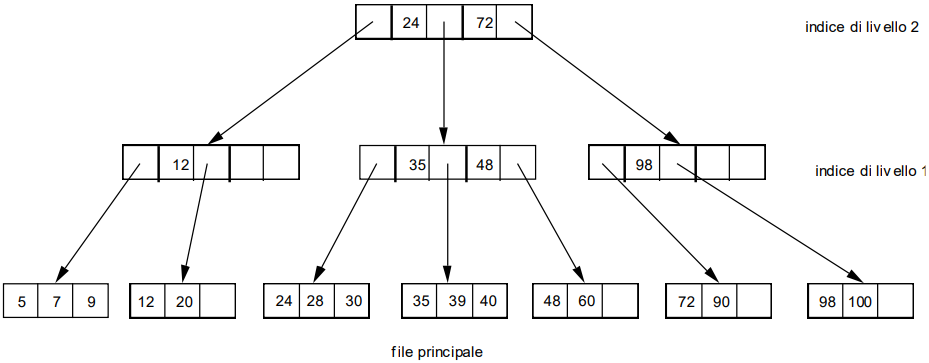
\includegraphics[width=\linewidth]{btree.png}
            \caption{Esempio di B-Tree}
        \end{figure}
        
\end{itemize}

\section{Concorrenza}

\textbf{Definizione} Una transazione è l'esecuzione di una parte di programma che interagisce con la base di dati, esse devono avere le seguenti priorità:
\begin{itemize}
    \item \textbf{Atomicità}

        La transazione deve essere eseguita completamente o per nulla.
    
    \item \textbf{Consistenza}

        Il DB non deve violare vincoli di integrità prima e dopo la transazione.
    
    \item \textbf{Isolamento}

        Ogni transazione deve essere indipendente dalle altre.
    
    \item \textbf{Durabilità}

        Non devono perdersi i cambiamenti apportati.\newline
    
\end{itemize}

\noindent\textbf{Definizione} La schedule di un insieme di transazioni è seriale se si ottiene permutando le transazioni, risulta sempre corretta.\newline

\noindent\textbf{Definizione} Una schedule non seriale è corretta se è serializzabile, ossia "equivale" ad una schedule seriale.\newline

\noindent\textbf{Definizione} Un item è un'unita con accesso controllato.\newline

\noindent Per evitare eventuali problemi si applica un lock sugli item:
\begin{itemize}
    \item \textbf{Binario}
    \item \textbf{A 3 valori}

        Si aggiunge un altro tipo di lock che permette ad altri di leggere l'item ma non di modificarlo.
    
\end{itemize}

\subsection{Stallo}

\textbf{Definizione} Il punto di commit di una transazione è il punto in cui:
\begin{itemize}
    \item Ha ottenuto tutti i lock necessari
    \item Ha effettuato tutti i calcoli
\end{itemize}
\noindent Se si trova a questo punto non può essere abortita.\newline

\noindent\textbf{Definizione} I dati sporchi sono quelli scritti da una transazione prima del suo punto di commit.\newline

\noindent In caso di deadlock si effettua il roll-back di una delle transazioni coinvolte, ossia:
\begin{itemize}
    \item La transazione viene abortita
    \item I suoi effetti sui dati vengono annullati
    \item Tutti i suoi lock vengono rilasciati\newline
\end{itemize}

\noindent Con il procedimento precedente diventa problematica la situazione in cui altre transazioni abbiano letto i dati sporchi prodotti dalla transazione abortita, per risolvere totalmente il problema si usa il locking a due fasi stretto:
\begin{enumerate}
    \item Una transazione non scrive fino al suo punto di commit
    \item Una transazione non rilascia nessun lock fino alla fine della scrittura
\end{enumerate}

\newpage
 
\part{}

\section{FOL}

\subsection{Sintassi}

L'alfabeto della logica del primo ordine è formato da:
\begin{itemize}
    \item Un insieme di variabili $V$
    \item Un insieme di simboli di funzione $F$, ognuno con la sua arità
    \item Un insieme di simboli di predicato $P$, ognuno con la sua arità ($=/2\text{\hspace{2pt}}\in P$)
    \item I connettivi logici ($\neg,\wedge,\vee,\rightarrow,\iff$)
    \item I quantificatori $\forall,\exists$
    \item I simboli ( ) ,
\end{itemize}

\noindent\rule{\textwidth}{0.5pt}

\noindent Esempi:
\begin{itemize}
    \item Funzione
        \begin{itemize}
            \item succ/1, succ(X) è il numero naturale successore di X
            \item zero/0, il numero 0 (arità 0 = simbolo di costante)
            \item padre/1, padre(X) è il padre della persona X
        \end{itemize}
    \item Predicato
        \begin{itemize}
            \item doppio/2, doppio(X,Y) indica che Y è il doppio di X
            \item uomo/1, uomo(X) indica che X è un uomo
            \item somma/3, somma(X,Y,Z) indica che Z=X+Y
        \end{itemize}
\end{itemize}

\noindent\rule{\textwidth}{0.5pt}\newline

\noindent Partendo dall'alfabeto si può definire il linguaggio della FOL, si procede in modo induttivo su 2 passi:
\begin{enumerate}
    \item Si definisce il linguaggio dei termini

        \vspace{5pt}

        L'insieme dei termini è definito induttivamente come:
            \begin{enumerate}
                \item Ogni variabile in $V$ è un termine
                \item Ogni simbolo di costante in $F$ è un termine
                \item $f/n\in F\wedge n>0\wedge (t_1,\ldots,t_n\text{ sono termini})\Rightarrow f(t_1,\ldots,t_n)$ è un termine
            \end{enumerate}

    \newpage
        
    \item Si definisce il linguaggio delle formule (usando il precedente)

        \vspace{5pt}

        L'insieme delle formule è definito induttivamente come:
            \begin{enumerate}
                \item $p/n\text{ è predicato}\wedge t_1,\ldots,t_n\text{ sono termini}\Rightarrow p(t_1,\ldots,t_n)$ è una formula (atomica)
                \item Se $\phi,\epsilon$ sono formule lo sono anche:
                    \begin{itemize}
                        \item $(\phi)$
                        \item $\neg\phi$
                        \item $\phi\wedge\epsilon$
                        \item $\phi\vee\epsilon$
                        \item $\phi\rightarrow\epsilon$
                        \item $\phi\iff\epsilon$
                    \end{itemize}
                \item Se $\phi$ è una formula e $X$ è una variabile sono formule:
                    \begin{itemize}
                        \item $\forall X\ \ \phi$
                        \item $\exists X\ \ \phi$
                    \end{itemize}
            \end{enumerate}
\end{enumerate}

\noindent\rule{\textwidth}{0.5pt}

\noindent Esempi:
\begin{itemize}
    \item $F=\{zero/0,succ/1,padre/1\}$

        Alcuni termini sono:
            \begin{itemize}
                \item $zero$
                \item $var$ (una variabile)
                \item $succ(zero)$
                \item $succ(succ(succ(padre(var))))$
            \end{itemize}

    \item $P=\{doppio/2,somma/3,mortale/1\}$ ed $F$

        Alcune formule sono:
            \begin{itemize}
                \item $\forall\ X\ \ mortale(X)$
                \item $doppio(succ(zero),X)$
                \item $(padre(X)=Z)\rightarrow(mortale(Z))\text{  (l'uguale non si scrive come gli altri predicati per comodità)}$ 
                \item $\forall X\ \exists Y \ doppio(X,Y)$\newline
            \end{itemize}

        Alcune sequenze di simboli non formule sono:
            \begin{itemize}
                \item $X\wedge Y$ (2 termini)
                \item $succ(zero)$ (termine)
                \item $mortale(mortale(X))$ (predicato dentro predicato)
                \item $padre(doppio(X,Z))$ (predicato dentro termine)
                \item $\exists zero \ \ mortale(zero)$ ($zero$ non è una variabile)
            \end{itemize}
\end{itemize}

\noindent\rule{\textwidth}{0.5pt}

\subsection{Semantica}

La semantica definisce il significato di una formula logica (la sua verità), in FOL ci sono 2 livelli sintattici quindi bisogna dare 2 concetti di valutazione:
\begin{itemize}
    \item Dei termini
            \begin{itemize}
                \item \textbf{Atomici}
                        \begin{itemize}
                \item \textbf{Pre-interpretazione}

                    \vspace{5pt}

                    Una pre-interpretazione è data da:
                        \begin{itemize}
                            \item Un insieme $D\neq\emptyset$ detto dominio di interpretazione
                            \item La funzione totale $PreI:D^n\rightarrow D:f/n\rightarrow d\in D$
                        \end{itemize}
                
                \item \textbf{Assegnamento di variabili}

                    \vspace{5pt}

                    Un assegnamento per $PreI$ è la funzione $S:V\rightarrow D$

            \end{itemize}
            \item \textbf{Complessi}

            \vspace{5pt}

            Dato $T$ insieme dei termini. Si definisce la funzione: 
            $$pre-eval^{PreI,S}:T\rightarrow D\ \ \text{ (indicata con }pe)$$ 
            
            Come:
                \begin{itemize}
                    \item $X\text{ è variabile}\Rightarrow pe(X)=S(X)$
                    \item $c\text{ simbolo di costante}\Rightarrow pe(c)=PreI(c)$
                    \item $pe(f(t_1,\ldots,t_n))=PreI(f(pe(t_1),\ldots,pe(t_n)))$
                \end{itemize}
            
        \end{itemize}

    \item Delle formule
            \begin{itemize}
                \item \textbf{Atomiche}
                        \begin{itemize}
                \item \textbf{Interpretazione}

                    Una funzione che associa a $p/n$ una relazione $I(p)\subseteq \underbrace{D\times\ldots\times D}_{\text{n volte}}$


                    Per l'uguale risulta $\{(d,d)\ |\ d\in D\}$
                
            \end{itemize}
            \item \textbf{Complesse}

                Dato $\phi$ insieme delle formule. Si definisce la formula:
                $$eval^{I,S}:\phi\rightarrow \{vero(1),falso(0)\}\ \ \text{ (indicata con }e)$$ 

                Come:
                \begin{itemize}
                    \item $e(p(t_1,\ldots,t_n))=I(p(pe(t_1),\ldots,pe(t_n)))$
                    \item Se $\phi, \epsilon$ sono formule:
                        \begin{itemize}
                            \item $e((\phi))=e(\phi)$
                            \item $e(\neg\phi)=1\text{ se }e(\phi)=0,\ 1$ altr.
                            \item $e(\phi\wedge\epsilon)=1\text{ se }e(\phi)=e(\epsilon)=1,\ 0$ altr.
                            \item $e(\phi\vee\epsilon)=1\text{ se }e(\phi)=1 \text{ o }e(\epsilon)=1,\ 0$ altr.
                            \item $e(\phi\rightarrow\epsilon)=e(\neg\phi\vee \epsilon)$
                            \item $e(\phi\iff\epsilon)=e((\phi\rightarrow\epsilon)\wedge(\epsilon\rightarrow\phi))$
                        \end{itemize}

                    \item $e(\exists V\ \phi)=1\text{ se esiste }d\in D\ |\ e^{I,S[V/d]}(\phi)=1,\ 0$ altr.

                    \item $e(\forall V\ \phi)=1\text{ se per ogni }d\in D\ e^{I,S[V/d]}(\phi)=1,\ 0$ altr.
                            
                \end{itemize}
             
        \end{itemize}

\end{itemize}

 ($S[X/d]$ indica l'assegnamento $S$ eccettuato il fatto che ad $X$ si assegna $d$)

\noindent\rule{\textwidth}{0.5pt}

Esempio:
$$S(X)=3\wedge S(Y)=4\Rightarrow S[Y/9](X)=3\wedge S[Y/9]=9$$

\noindent\rule{\textwidth}{0.5pt}\newline

\noindent\textbf{Definizione} Una formula è detta chiusa se tutte le sue variabili sono quantificate, il suo valore di verità dipende dall'interpretazione usata e conseguentemente dal dominio.\newline

\noindent\textbf{Definizione} Il modello di una formula chiusa $\phi$ è un'interpretazione $M$ per cui $e^{M,S}(\phi)=vero$ per qualsiasi assegnamento $S$ ($M |=\phi$).\newline

\noindent\textbf{Definizione} Una formula $\phi$ è definita:
\begin{itemize}
    \item \textbf{Soddisfacibile}

        $$\exists I,S\ \ e^{I,S}(\phi)=vero$$

    \item \textbf{Insoddisfacibile}

        $$\forall\  I,S\ \ e^{I,S}(\phi)=falso$$

    \item \textbf{Valida}

        $$\forall\ I,S\ \ e^{I,S}(\phi)=vero$$\newline
    
\end{itemize}

\noindent Convenzionalmente si usa la seguente precedenza per connettivi e quantificatori:
\begin{enumerate}
    \item $\neg$
    \item $\wedge,\vee$
    \item $\forall,\exists$
    \item $\rightarrow$
\end{enumerate}

\newpage

\subsection{Esempio completo}

\noindent\rule{\textwidth}{0.5pt}

\begin{itemize}
    \item $F=\{zero/0,succ/1\}$
    \item $P=\{doppio/2,somma/3\}$
    \item $V=\{X,Y,Z\}$
    \item Pre-interpretazione $PreNAT$
        \begin{itemize}
            \item $D=\mathbf{N}$
            \item $PreNAT(zero)=0$
            \item $PreNAT(succ):D\rightarrow D:PreNAT(0)=1,PreNAT(1)=2,\ldots$
        \end{itemize}
    \item Assegnamento $W$
        \begin{itemize}
            \item $W(X)=3$
            \item $W(Y)=6$
            \item $W(Z)=4$
        \end{itemize}

    \item Valutazione termini $pe$
        \begin{itemize}
            \item $pe(zero)=PreNAT(zero)=0$
            \item Esempio: \begin{equation}
                \nonumber
                \begin{split}
                    pe(succ(succ(X)))&=PreNAT(succ(pe(succ(X))))\\
                    &=PreNAT(succ(PreNAT(succ(pe(X)))))\\
                    &=PreNAT(succ(PreNAT(succ(W(X)))))\\
                    &=PreNAT(succ(PreNAT(succ(3))))=5
                \end{split}
            \end{equation}
        \end{itemize}

    \item Interpretazione $NAT$
        \begin{itemize}
            \item $NAT(doppio)=\{(x,y)\ |\ y=2x\}$
            \item $NAT(somma)=\{(x,y,z)\ |\ z=x+y\}$
        \end{itemize}

    \item Valutazione $e$

\end{itemize}

Esempi di valutazione:

\begin{equation}
    \nonumber
    \begin{split}
        &e(doppio(succ(succ(zero)),X))=\\
        &=NAT(doppio(pe(succ(succ(zero))),pe(X)))\\
        &=NAT(doppio(PreNAT(succ(pe(succ(zero)))),W(X)))\\
        &=NAT(doppio(PreNAT(succ(PreNAT(succ(pe(zero))))),3))\\
        &=NAT(doppio(PreNAT(succ(PreNAT(succ(PreNAT(zero))))),3))\\
        &=NAT(doppio(PreNAT(succ(PreNAT(succ(0)))),3))\\
        &=NAT(doppio(PreNAT(succ(1)),3))\\
        &=NAT(doppio(2,3))=falso\\
    \end{split}  
\end{equation}

\begin{equation}
    \nonumber
    \begin{split}
        &e(somma(succ(zero),zero,succ(zero)))=\\
        &=NAT(somma(pe(succ(zero)),pe(zero),pe(succ(zero))))\\
        &=NAT(somma(PreNAT(succ(pe(zero))),PreNAT(zero),PreNAT(succ(pe(zero)))))\\
        &=NAT(somma(PreNAT(succ(0)),0,PreNAT(succ(zero))))\\
        &=NAT(somma(1,0,1))=vero\\ 
    \end{split}  
\end{equation}

\begin{equation}
    \nonumber
    \begin{split}
        e(\forall X\ \ doppio(succ(succ(zero))),X)&=e^{NAT,W[X/d]}(doppio(succ(succ(zero)),X))\\
        &=e^{NAT,W[X/d]}(doppio(2,X))= falso \text{ (dato }d=1)\\
    \end{split}  
\end{equation}

\begin{equation}
    \nonumber
    \begin{split}
        &e(\forall X\ \exists Y\ \ doppio(X,Y)) \text{ essendo chiusa risulta vera data l'interpretazione di $doppio$ e $D=\mathbf{N}$}\\
        & \text{Invertendo $X,Y$ nei quantificatori diventa falsa, infatti non esiste un numero in $\mathbf{N}$ il cui doppio è 3}
    \end{split}  
\end{equation}

\noindent\rule{\textwidth}{0.5pt}

\end{document}
